\documentclass[polish,polish,a4paper]{article}
\usepackage[polish]{babel}
\usepackage[T1]{fontenc}
\usepackage[utf8]{inputenc}
\usepackage{pslatex}
\usepackage{pgfplots}
\usepackage{circuitikz} 
\usepackage{setspace}
\usepackage{caption}
\usepackage{amssymb}
\usepackage{amsmath}
%\usetikzlibrary{circuits.ee.IEC}
\usepackage{anysize}
\usepackage{graphicx}
\usepackage{hyperref}
\usepackage{float}
\usepackage{color}
\hypersetup{
	colorlinks=true,
	linkcolor=blue,
	filecolor=magenta,      
	urlcolor=cyan,
}

\marginsize{2.5cm}{2.5cm}{2cm}{2cm}

\newcommand{\PRzFieldDsc}[1]{\sffamily\bfseries\scriptsize #1}
\newcommand{\PRzFieldCnt}[1]{\textit{#1}}
\newcommand{\PRzHeading}[8]{
	%% #1 - nazwa laboratorium
	%% #2 - kierunek 
	%% #3 - specjalność 
	%% #4 - rok studiów 
	%% #5 - symbol grupy lab.
	%% #6 - temat 
	%% #7 - numer lab.
	%% #8 - skład grupy ćwiczeniowej
	
	\begin{center}
		\begin{tabular}{ p{0.32\textwidth} p{0.15\textwidth} p{0.15\textwidth} p{0.12\textwidth} p{0.12\textwidth} }
			
			&   &   &   &   \\
			\hline
			\multicolumn{5}{|c|}{}\\[-1ex]
			\multicolumn{5}{|c|}{{\LARGE #1}}\\
			\multicolumn{5}{|c|}{}\\[-1ex]
			
			\hline
			\multicolumn{1}{|l|}{\PRzFieldDsc{Kierunek}}	& \multicolumn{1}{|l|}{\PRzFieldDsc{Specjalność}}	& \multicolumn{1}{|l|}{\PRzFieldDsc{Rok studiów}}	& \multicolumn{2}{|l|}{\PRzFieldDsc{Symbol grupy lab.}} \\
			\multicolumn{1}{|c|}{\PRzFieldCnt{#2}}		& \multicolumn{1}{|c|}{\PRzFieldCnt{#3}}		& \multicolumn{1}{|c|}{\PRzFieldCnt{#4}}		& \multicolumn{2}{|c|}{\PRzFieldCnt{#5}} \\
			
			\hline
			\multicolumn{4}{|l|}{\PRzFieldDsc{Temat Laboratorium}}		& \multicolumn{1}{|l|}{\PRzFieldDsc{Numer lab.}} \\
			\multicolumn{4}{|c|}{\PRzFieldCnt{#6}}				& \multicolumn{1}{|c|}{\PRzFieldCnt{#7}} \\
			
			\hline
			\multicolumn{5}{|l|}{\PRzFieldDsc{Skład grupy ćwiczeniowej oraz numery indeksów}}\\
			\multicolumn{5}{|c|}{\PRzFieldCnt{#8}}\\
			
			\hline
			\multicolumn{3}{|l|}{\PRzFieldDsc{Uwagi}}	& \multicolumn{2}{|l|}{\PRzFieldDsc{Ocena}} \\
			\multicolumn{3}{|c|}{\PRzFieldCnt{\ }}		& \multicolumn{2}{|c|}{\PRzFieldCnt{\ }} \\
			
			\hline
		\end{tabular}
	\end{center}
}



\begin{document}


	\PRzHeading{Laboratorium Podstaw Elektroniki}{Informatyka}{--}{I}{I3}{Tranzystory}{5}{Piotr Więtczak(132339), Robert Ciemny(136693), Kamil Basiukajc(136681)}
\section{Charakterystyka bramkowa nMOS}

\subsection{Cel zadania}

Wyznaczenie empirycznej zależności pomiędzy sygnałem sterującym a sterowanym.

\subsection{Przebieg zadania}

Przy pomocy poniższego układu dokonano serii pomiarów wartości prądu drenu $I_{D}$ w zależności od napięcia $U_{GS}$ zmienianego w zakresie $<0..5> V$. Po odkryciu lawinowego wzrostu przepływu prądu w zakresie $<2.0,2.5>$ zagęszczono punkty pomiarowe w tym obszarze. Wyniki pomiarów przedstawiono w poniższej tabeli.


%%  rys 1.6.
\begin{figure}[H]
	\begin{equation*}
	\begin{circuitikz}[american]
	\draw
	(0,0) to (6,0)
	(0,0) to[V,v=$5V$] (0,3)
	to (0,5)
	to [esource](3,5)
	to [european resistor, l=$R_{1}$, a=$1k\Omega$](6,5)
	(6,3) node[nmos] (mos) {}
	(mos.drain) node[anchor = west] {D}
	(mos.source) node[anchor = west] {S}
	(mos.gate) node[anchor = south] {G}
	(6,0) to (mos.source)
	(mos.drain) to (6,5)
	(mos.gate) to (3,3)
	(3,0) to [V,v=$0..5V$] (3,3)
	(4.5,0) to [esource] (4.5,3)
	(4.5,1.45) node[anchor = mid] {V}
	(5,0.5) to (5,2.5)
	node[currarrow,rotate = 90] {}
	(5.5,1.5) node[anchor = mid] {$ U_{GS} $}
	(1.5,4.95) node[anchor = mid] {mA}
	(3,0) node[ground] {};
	\end{circuitikz}
	\end{equation*}
	\captionof{figure}{Układ do badania charakterystyki bramkowej tranzystora nMOS}
\end{figure}

%tabelka	
	\begin{figure}[H]
\begin{spacing}{1.5}
		\begin{equation*}
\begin{array}{|r|r|r|}
\hline
\multicolumn{1}{|c|}{ $Napięcie$}&\multicolumn{1}{c|}{ $Napięcie$}&\multicolumn{1}{|c|}{I_{D}}\\
\multicolumn{1}{|c|}{ $źródła $ [V] }&\multicolumn{1}{|c|}{U_{GS}$ $[V]}&\multicolumn{1}{|c|}{[mA]}\\\hline
0&0&0.000\\
0.5&0.491&0.000\\
1.0&1.120&0.000\\
1.5&1.459&0.000\\
2.0&1.982&1.360\\
2.1&2.043&3.641\\
2.2&2.182&4.905\\
2.3&2.293&4.699\\
2.4&2.356&4.987\\
2.5&2.488&4.986\\
3.0&2.988&5.000\\
3.5&3.431&5.009\\
4.0&4.051&5.011\\
4.5&4.492&5.014\\
5.0&4.880&5.015\\
\hline
\end{array}
\end{equation*}
\end{spacing}
\captionof{table}{Tabela przedstawiająca wyniki pomiarów}
	\end{figure}

	%%WYKRES 
\begin{figure}[H]
	
	\centering
	\begin{tikzpicture}
	\begin{axis}[
	width=0.9\textwidth,
	height = 0.5\textwidth,
	title={Wykres przedstawiający wyniki pomiarów},
	ylabel={wartości prądu drenu $I_{d}$ $[mA]$},
	xlabel ={wartości napięcia $U_{GS}$ $[V]$},
	%
	scaled x ticks = false,
	xtick distance = 0.5,
	x tick label style={/pgf/number format/fixed},
	xticklabel style = {rotate= 90},
	x label style={at={(axis description cs:0.5,-0.15)},anchor=north},
	%%
	ytick distance = 1,
	scaled y ticks = false,
	y tick label style={/pgf/number format/fixed},
	y label style={at={(axis description cs:-0.05,0.85)},anchor=east},
	%%
	legend pos=north west,
	ymajorgrids=true,
	grid style=dashed,
	]
	%%
	\addplot[
	color=black,
	mark=*,
	]
	coordinates {
(0,0.000)(0.491,0.000)(1.120,0.000)(1.459,0.000)(1.982,1.360)(2.043,3.641)(2.182,4.905)(2.293,4.699)(2.356,4.987)(2.488,4.986)(2.988,5.000)(3.431,5.009)(4.051,5.011)(4.492,5.014)(4.880,5.015)
	};
	%%
	\addplot[
	color=red,
	]
	coordinates {
		(2,-0.5)(2,5.5)
	};
	\legend{
		$I_{D} -pomiary$,
		$U_{th}$
	}
	%%
	\end{axis}
	\end{tikzpicture}
\end{figure}


\subsection{Wniosek }
Przy niskim napięciu $U_{GS}$ wartość $I_{D}$ przyjmuje $0mA$ wraz z wzrostem napięcia $U_{GS}$ wartość $I_{D}$ początkowo dalej utrzymuje się na poziomie zerowym, aby przed osiągnięciem napięcia $U_{th}$ zacząć lawinowo wzrastać by po jego przekroczeniu ustabilizować się na poziomie około $5mA$. 
\section{Charakterystyka bramkowa pMOS}
\subsection{Cel zadania}
Wykazanie dualizmu między działaniem tranzystora pMOS względem nMOS.
\subsection{Przebieg zadania}



Przy pomocy poniższego układu dokonano serii pomiarów wartości prądu $I_{D}$ w zależności od napięcia wytwarzanego przez zasilacz. Po odkryciu lawinowego wzrostu prądu drenu w zakresie $<2.0,3.0>$ zagęszczono punkty pomiarowe w tym obszarze.

Na podstawie uzyskanych wyników obliczono wartości napięć bramka-źródło dla tranzystora pMOS korzystając z napięciowego prawa Kirchhoffa: $U_{GS} = -(U_{SS}-U_{1})$ dla $U_{SS} = 5V$.

%%  rys 1.7.
\begin{figure}[H]
	\begin{equation*}
	\begin{circuitikz}[american]
	\draw
	(-1.5,1) to (-1.5,4)
	node[currarrow, rotate = 90] {}
	(-2,2.5) node[anchor = mid] {$U_{SS}$}
	(0,0) to (4.5,0)
	(4.5,0) to [esource] (8,0)
	(0,0) to[V,v=$5V$] (0,3)
	to (0,5)
	to (8,5)
	(8,3) node[pmos] (mos) {}
	(mos.drain) node[anchor = west] {D}
	(mos.source) node[anchor = west] {S}
	(mos.gate) node[anchor = south] {G}
	(8,0) to [european resistor, l=$R_{7}$, a=$1k\Omega$] (mos.drain)
	(mos.source) to (8,5)
	(mos.gate) to (3,3)
	(3,0) to [V,v=$0..5V$] (3,3)
	(4.5,0) to [esource] (4.5,3)
	(4.5,1.45) node[anchor = mid] {V}
	(5,0.5) to (5,2.5)
	node[currarrow, rotate = 90] {}
		(5.5,1.5) node[anchor = mid] {$ U_{1} $}
		(7.5,4.5) to (7.5,3.7)
	node[currarrow, rotate = -90] {}
	(7.0,3.9)	node[anchor = mid] {$U_{GS}$}

	(3,0) node[ground] {}
	(6.25,0) node[anchor = mid] {mA};
	\end{circuitikz}
	\end{equation*}
	\captionof{figure}{Układ do badania charakterystyki bramkowej tranzystora pMOS}
\end{figure}

%tabelka
	\begin{figure}[H]
	\begin{spacing}{1.3}
		\begin{equation*}
		\begin{array}{|r|r|r|r|}
		\hline
		\multicolumn{1}{|c|}{ $Napięcie$}&\multicolumn{1}{|c|}{ $Napięcie$}&\multicolumn{1}{|c|}{ $Napięcie$}&\multicolumn{1}{|c|}{I_{D}}\\
		\multicolumn{1}{|c|}{  V_{1}$ $[V]}&\multicolumn{1}{|c|}{ U_{1}$ $[V]}&\multicolumn{1}{|c|}{ U_{GS}$ $[V]}&\multicolumn{1}{|c|}{[mA]}\\\hline
0.0&0.000&-5.000&5.000\\
0.5&0.473&-4.527&5.000\\
1.0&0.982&-4.018&5.000\\
1.5&1.495&-3.505&5.000\\
2.0&1.971&-3.029&4.973\\
2.1&2.082&-2.918&4.950\\
2.2&2.191&-2.809&4.901\\
2.3&2.289&-2.711&4.721\\
2.4&2.376&-2.624&4.166\\
2.5&2.431&-2.569&2.793\\
2.6&2.548&-2.452&1.050\\
2.7&2.674&-2.326&0.563\\
2.8&2.793&-2.207&0.249\\
2.9&2.891&-2.109&0.044\\
3.0&2.975&-2.025&0.023\\
3.5&3.483&-1.517&0.000\\
4.0&3.974&-1.026&0.000\\
4.5&4.431&-0.569&0.000\\
5.0&4.982&-0.018&0.000\\
\hline
		\end{array}
		\end{equation*}
	\end{spacing}
\end{figure}

	%%WYKRES 
\begin{figure}[H]
	
	\centering
	\begin{tikzpicture}
	\begin{axis}[
	width=0.9\textwidth,
	height = 0.5\textwidth,
	title={Czasy obliczania etykiet dla grafów},
	xlabel={Liczba wierzchołków},
	ylabel={Czas obliczania w misekundach},
	%
	scaled x ticks = false,
	xtick distance = 0.5,
	x tick label style={/pgf/number format/fixed},
	xticklabel style = {rotate= 90},
	x label style={at={(axis description cs:0.5,-0.15)},anchor=north},
	%%
	ytick distance = 1,
	scaled y ticks = false,
	y tick label style={/pgf/number format/fixed},
	y label style={at={(axis description cs:-0.05,0.85)},anchor=east},
	%%
	legend pos=north east,
	ymajorgrids=true,
	grid style=dashed,
	]
	%%
	\addplot[
	color=black,
	mark=*,
	]
	coordinates {
(0.000,5.000)(0.473,5.000)(0.982,5.000)(1.495,5.000)(1.971,4.973)(2.082,4.950)(2.191,4.901)(2.289,4.721)(2.376,4.166)(2.431,2.793)(2.548,1.050)(2.674,0.563)(2.793,0.249)(2.891,0.044)(2.975,0.023)(3.483,0.000)(3.974,0.000)(4.431,0.000)(4.982,0.000)


	};
	%%
	\addplot[
	color=red,
	]
	coordinates {
		(2.4,-0.5)(2.4,5.5)
		
	};
	\legend{
		$I_{D} -pomiary$,
		$U_{th}$,
	}
	%%
	\end{axis}
	\end{tikzpicture}
\end{figure}

\section{Charakterystyka drenowa nMOS}

\subsection*{Cel zadania}
Analiza zależności między wartością napięcia $D_{DS}$, a wartością prądu $I_{D}$.


\subsection*{Przebieg zadania}

Po przygotowaniu poniższego schematu zmierzono napięcie Bramka-Źródło $U_{GS}$ które wyniosło $4.978V$. Następnie wykonano serię pomiarów wartości prądu drenu $I_{D}$ w zależności od napięcia Dren-Źródło $U_{DS}$. Dla napięcia zasilania zmienianego w zakresie $ <0..10>V $.

%%  rys 1.8.
\begin{figure}[H]
	\begin{equation*}
	\begin{circuitikz}[american]
	\draw
	(0,0) to (6,0)
	(0,0) to[V,v=$0..10V$] (0,3)
	to (0,5)
	to [esource](3,5)
	to [european resistor, l=$R_{2}$, a=$1k\Omega$](6,5)
	(6,3) node[nmos] (mos) {}
	(mos.drain) node[anchor = west] {D}
	(mos.source) node[anchor = west] {S}
	(mos.gate) node[anchor = south] {G}
	(6,0) to (mos.source)
	(mos.drain) to (6,5)
	(mos.gate) to (3,3)
	(3,0) to [V,v=$5V$] (3,3)
	(1.5,4.95) node[anchor = mid] {mA}
	(3,0) node[ground] {}
	(6,0) to (7.5,0)
	to [esource] (7.5,5)
	to(6,5)
	(7.5,2.45) node[anchor = mid] {V}
	(6.5,1.5) to (6.5,4.5)
	node[currarrow, rotate = 90] {}
	(6.9,3.2) node[anchor = mid] {$U_{DS}$};
	
	\end{circuitikz}
	\end{equation*}
	\captionof{figure}{Układ do badania charakterystyki drenowej tranzystora nMOS}
\end{figure}

%tabelka	
\begin{figure}[H]
	\begin{spacing}{1.3}
		\begin{equation*}
		\begin{array}{|r|r|r|}
		\hline
		\multicolumn{1}{|c|}{ $Napięcie$}&
		\multicolumn{1}{c|}{ $Napięcie$}&
		\multicolumn{1}{c|}{I_{D}}\\
		\multicolumn{1}{|c|}{ U_{IN}$ $[V]}&
		\multicolumn{1}{c|}{ U_{DS}$ $[V]}&
		\multicolumn{1}{c|}{[mA]}\\
		\hline
0&0&0\\
1&1.179&1.851\\
2&2.171&3.511\\
3&3.271&5.018\\
4&4.138&6.658\\
5&5.121&7.912\\
6&6.105&9.551\\
7&7.201&11.325\\
8&8.137&12.670\\
9&9.238&14.342\\
10&10.154&15.785\\
\hline
		\end{array}
		\end{equation*}
	\end{spacing}
\captionof{table}{Tabelea prezentująca wyniki}
\end{figure}


Następnie przygotowano zestaw pomiarowy według poniższego schematu i zmierzono napięcie Bramka-Źródło $U_{DS}$ które wyniosło $2.732V$. Wykonano serię pomiarów wartości prądu drenu $I_{D}$ w zależności od napięcia Dren-Źródło $U_{DS}$. Dla napięcia zasilania zmienianego w zakresie $ <0..10>V $.

%%  rys 1.9.
\begin{figure}[H]
	\begin{equation*}
	\begin{circuitikz}[american]
	\draw
	(0,0) to (6,0)
	(0,0) to[V,v=$0..10V$] (0,3)
	to (0,5)
	to [esource](3,5)
	to [european resistor, l=$R_{3}$, a=$1k\Omega$](6,5)
	(6,3) node[nmos] (mos) {}
	(mos.drain) node[anchor = west] {D}
	(mos.source) node[anchor = west] {S}
	(mos.gate) node[anchor = south] {G}
	(6,0) to (mos.source)
	(mos.drain) to (6,5)
	(mos.gate) to (5,3)
	(3,3) to [european resistor, l=$R_{4}$, a= $1k\Omega$] (5,3)
	(5,0) to [european resistor, l=$R_{5}$ , a=$1k\Omega$] (5,3)
	(3,0) to [V,v=$5V$] (3,3)
	(1.5,4.95) node[anchor = mid] {mA}
	(3,0) node[ground] {}
	(6,0) to (7.5,0)
	to [esource] (7.5,5)
	to(6,5)
	(7.5,2.45) node[anchor = mid] {V};
	\end{circuitikz}
	\end{equation*}
	\captionof{figure}{Układ do badania charakterystyki drenowej dla obniżonego napięcia bramki}
\end{figure}


%tabelka	
\begin{figure}[H]
	\begin{spacing}{1.3}
		\begin{equation*}
		\begin{array}{|r|r|r|}
		\hline
		\multicolumn{1}{|c|}{ $Napięcie$}&
		\multicolumn{1}{c|}{ $Napięcie$}&
		\multicolumn{1}{c|}{I_{D}}\\
		\multicolumn{1}{|c|}{ U_{IN}$ $[V]}&
		\multicolumn{1}{c|}{ U_{DS}$ $[V]}&
		\multicolumn{1}{c|}{[mA]}\\
		\hline
0&0&0\\
1&1.132&15.011\\
2&2.129&31.623\\
3&3.098&46.258\\
4&4.095&67.012\\
5&5.076&92.025\\
6&6.082&125.895\\
7&7.023&183.756\\
8&7.826&322.326\\
9&8.175&756.497\\
10&8.567&1465.127\\

		\hline
		\end{array}
		\end{equation*}
	\end{spacing}
\end{figure}



%%WYKRES 
\begin{figure}[H]
	
	\centering
	\begin{tikzpicture}
	\begin{axis}[
	width=0.9\textwidth,
	height = 0.5\textwidth,
	title={Czasy obliczania etykiet dla grafów},
	xlabel={Liczba wierzchołków},
	ylabel={Czas obliczania w misekundach},
	%
	scaled x ticks = false,
	xtick distance = 0.5,
	x tick label style={/pgf/number format/fixed},
	xticklabel style = {rotate= 90},
	x label style={at={(axis description cs:0.5,-0.15)},anchor=north},
	%%
	ytick distance = 100,
	scaled y ticks = false,
	y tick label style={/pgf/number format/fixed},
	y label style={at={(axis description cs:-0.05,0.85)},anchor=east},
	%%
	legend pos=north west,
	ymajorgrids=true,
	grid style=dashed,
	]
	%%
	\addplot[
	color=black,
	mark=*,
	]
	coordinates {
		(0,0)(1.179,1.851)(2.171,3.511)(3.271,5.018)(4.138,6.658)(5.121,7.912)(6.105,9.551)(7.201,11.325)(8.137,12.670)(9.238,14.342)(10.154,15.785)
	};
	%%
	\addplot[
	color=blue,
	mark=triangle,
	]
	coordinates {
		(0,0)(1.132,15.011)(2.129,31.623)(3.098,46.258)(4.095,67.012)(5.076,92.025)(6.082,125.895)(7.023,183.756)(7.826,322.326)(8.175,756.497)(8.567,1465.127)
		
		
	};
	\legend{
		$I_{D} -$ dla $U_{SG} = 4.986V$,
		$I_{D} -$ dla $U_{SG} = 2.723V$,
	}
	%%
	\end{axis}
	\end{tikzpicture}
\end{figure}

\subsection{Wnioski}

Wraz z wzrostem napięcia $U_{DS}$ wzrasta wartość $I_{D}$
Dla obniżonego napięcia Bramka-Źródło wartość prądu drenu wzrasta szybciej.  

\section{Charakterystyka drenowa pMOS}

\subsection*{Cel zadania}
Analiza zależności między wartością napięcia $D_{DS}$, a wartością prądu $I_{D}$.


\subsection*{Przebieg zadania}

Po przygotowaniu poniższego schematu zmierzono napięcie Bramka-Źródło $U_{GS}$ które wyniosło $-4.986V$. Następnie wykonano serię pomiarów wartości prądu drenu $I_{D}$ w zależności od napięcia Dren-Źródło $U_{DS}$. Dla napięcia zasilania zmienianego w zakresie $ <0..10>V $.


%%  rys 1.10.
\begin{figure}[H]
	\begin{equation*}
	\begin{circuitikz}[american]
	\draw
	(-1,2) to (-1,4)
	node[currarrow, rotate=90] {}
	(-1.5,2.5) node[anchor = mid] {$U_{SD}$}
	(0,0) to (3,0)
	to [esource] (5,0)
	(4,0) node[anchor = mid] {mA}
	(0,0) to[V,v=$0..10V$] (0,3)
	to (0,5)
	to (5,5)
	(5,3) node[pmos] (mos) {}
	(mos.drain) node[anchor = west] {D}
	(mos.source) node[anchor = west] {S}
	(mos.gate) node[anchor = south] {G}
	(5,0) to [european resistor, l=$R_{6}$, a=$1k\Omega$] (mos.drain)
	(mos.source) to (5,5)
	(mos.gate) to (3,3)
	(3,0) to [V,v=$5V$] (3,3)
	(3,0) node[ground] {}
	(5,0) to (6.5,0)
	to [esource] (6.5,5)
	to (5,5)
	(6.5,2.45) node[anchor = mid] {V};
	\end{circuitikz}
	\end{equation*}
	\captionof{figure}{Układ do badania charakterystyki drenowej tranzystora pMOS}
\end{figure}


%tabelka	
\begin{figure}[H]
	\begin{spacing}{1.3}
		\begin{equation*}
		\begin{array}{|r|r|r|r|}
		\hline
		\multicolumn{1}{|c|}{ $Napięcie$}&
		\multicolumn{1}{c|}{ $Napięcie$}&
		\multicolumn{1}{c|}{ $Napięcie$}&
		\multicolumn{1}{c|}{I_{D}}\\
		\multicolumn{1}{|c|}{ U_{IN}$ $[V]}&
		\multicolumn{1}{c|}{ U_{GS}$ $[V]}&
		\multicolumn{1}{c|}{ U_{DS}$ $[mV]}&
		\multicolumn{1}{c|}{[mA]}\\
		\hline
0&4.87&0&0\\
1.139&3.689&-1138&0\\
2.198&2.685&-2239&0\\
3.127&1.759&-3147&0\\
4.191&0.721&-4155&0\\
5.211&-0.273&-5263&0\\
6.173&-1.246&-6162&0\\
7.124&-2.201&-7165&0\\
8.072&-3.148&-209.489&8.016\\
9.135&-4.218&-258.754&9.025\\
10.192&-5.286&-204.156&10.208\\
		\hline
		\end{array}
		\end{equation*}
	\end{spacing}
	\captionof{table}{Tabela prezentująca wyniki}
\end{figure}


Następnie złożono poniższy schemat i zbadano napięcie Bramka-Źródło $U_{GS}$ które wyniosło $-2.723V$. Następnie wykonano serię pomiarów wartości prądu drenu $I_{D}$ w zależności od napięcia Dren-Źródło $U_{DS}$. Dla napięcia zasilania zmienianego w zakresie $ <0..10>V $.

%%  rys 1.11.
\begin{figure}[H]
	\begin{equation*}
	\begin{circuitikz}[american]
	\draw
	(-1,2) to (-1,4)
	node[currarrow, rotate=90] {}
	(-1.5,2.5) node[anchor = mid] {$U_{SD}$}
	(0,0) to (5,0)
	to [esource] (7,0)
	(6,0) node[anchor = mid] {mA}
	(0,0) to[V,v=$0..10V$] (0,3)
	to (0,5)
	to (7,5)
	(7,3) node[pmos] (mos) {}
	(mos.drain) node[anchor = west] {D}
	(mos.source) node[anchor = west] {S}
	(mos.gate) node[anchor = south] {G}
	(7,0) to [european resistor, l =$R_{8}$ , a=$1k\Omega$](mos.drain)
	(mos.source) to (7,5)
	(mos.gate) to (5,3)
	(3,3) to [european resistor, l = $R_{9}$, a = $1k\Omega$] (5,3)
	(3,0) to [V,v=$5V$] (3,3)
	(5,0) to [european resistor, l = $R_{10}$, a = $1k\Omega$] (5,3)
	(3,0) node[ground] {}
	(7,0) to (8.5,0)
	to [esource] (8.5,5)
	to (7,5)
	(8.5,2.45) node[anchor = mid] {V};
	\end{circuitikz}
	\end{equation*}
	\captionof{figure}{Układ do badania charakterystyki drenowej dla obniżonego napięcia bramki pMOS}
\end{figure}


%tabelka	
\begin{figure}[H]
	\begin{spacing}{1.3}
		\begin{equation*}
		\begin{array}{|r|r|r|r|}
		\hline
		\multicolumn{1}{|c|}{ $Napięcie$}&
		\multicolumn{1}{c|}{ $Napięcie$}&
		\multicolumn{1}{c|}{ $Napięcie$}&
		\multicolumn{1}{c|}{I_{D}}\\
		\multicolumn{1}{|c|}{ U_{IN}$ $[V]}&
		\multicolumn{1}{c|}{ U_{GS}$ $[V]}&
		\multicolumn{1}{c|}{ U_{DS}$ $[mV]}&
		\multicolumn{1}{c|}{[mA]}\\
		\hline
0&2.456&0&0\\
1.315&1.126&-1289&0\\
2.115&0.326&-2145&0\\
3.198&-0.756&-3214&0\\
4.167&-1.715&-4128&0\\
5.081&-2.631&-263&4.826\\
6.112&-3.654&-52&6.195\\
7.097&-4.634&-45&7.182\\
8.012&-5.539&-40&8.098\\
9.008&-6.546&-38&9.136\\
10.021&-7.498&-34&10.185\\
		\hline
		\end{array}
		\end{equation*}
	\end{spacing}
	\captionof{table}{Tabelea prezentująca wyniki}
\end{figure}



%%WYKRES 
\begin{figure}[H]
	
	\centering
	\begin{tikzpicture}
	\begin{axis}[
	width=0.9\textwidth,
	height = 0.5\textwidth,
	title={Czasy obliczania etykiet dla grafów},
	xlabel={Liczba wierzchołków},
	ylabel={Czas obliczania w misekundach},
	%
	scaled x ticks = false,
	xtick distance = 250,
	x tick label style={/pgf/number format/fixed},
	xticklabel style = {rotate= 90},
	x label style={at={(axis description cs:0.5,-0.15)},anchor=north},
	%%
	ytick distance = 1,
	scaled y ticks = false,
	y tick label style={/pgf/number format/fixed},
	y label style={at={(axis description cs:-0.05,0.85)},anchor=east},
	%%
	legend pos=north west,
	ymajorgrids=true,
	grid style=dashed,
	]
	%%
	\addplot[
	color=black,
	mark=*,
	]
	coordinates {
(-7165,0)(-6162,0)(-5263,0)(-4155,0)(-3147,0)(-2239,0)(-1138,0)(-209.489,8.016)(-258.754,9.025)(-204.156,10.208)
	};
	%%
	\addplot[
	color=blue,
	mark=triangle,
	]
	coordinates {
(-2145,0)(-3214,0)(-4128,0)(-1289,0)(-263,4.826)(-52,6.195)(-45,7.182)(-40,8.098)(-38,9.136)(-34,10.185)	
	};
	\legend{
		pierwszy obwód,
		drugi obwód,
	}
	%%
	\end{axis}
	\end{tikzpicture}
\end{figure}



\subsection{Wnioski}

Dla wartości napięcia bramki bliższych wartości 0 wartość prądu $I_{D}$ osiąga wartości różne od zera. Wraz ze spadkiem napięcia bramki spada wartość prądu $I_{D}$, aby w pewnym momencie osiągnąć wartość 0 i dalej utrzymywać się na tej wartości.

\section{Tranzystor nMOS jako przełącznik}

\subsection{Cel zadania}
Użycie tranzystora nMOS jako przełącznika

\subsection{Przebieg zadania}
Przygotowano poniższy układ pomiarowy.

%%  rys 1.14.
\begin{figure}[H]
	\begin{equation*}
	\begin{circuitikz}[american]
	\draw
	(0,0) to (6,0)
	to [V,v=$10V$] (6,3)
	(6,3) to  [european resistor, a = $R_{11}$, l= $1k\Omega$](4,3)
	(2,3) to [leD-,invert,a=LED1] (4,3)
	(2,2) node[nmos] (mos) {}
	(mos.drain) node[anchor = east] {D}
	(mos.source) node[anchor = east] {S}
	(mos.gate) node[anchor = south] {G}
	(2,3) to (mos.drain)
	(2,0) to (mos.source)
	(mos.gate) to (0,2)
	(0,2) to [european resistor, a =$R_{12}$, l=$1M\Omega$] (0,0)
	(0,2) to [short, -*] (-1,2)
	(6,3) to (6,4.5)
	to (-1,4.5)
	to [short,-*] (-1,3)
	(-1,2.5) node[anchor = mid] {A-A};
	\end{circuitikz}
	\end{equation*}
	\captionof{figure}{Schemat układu do badania tranzystora nMOS w roli przełącznika}
\end{figure}

Następnie po podłączeniu napięcia zasilającego zwarto palcem zaciski obwodu oznaczone jako $ A-A $ i zaobserwowano przełączenie stanu diody.

\begin{figure}[H]
	\centering
	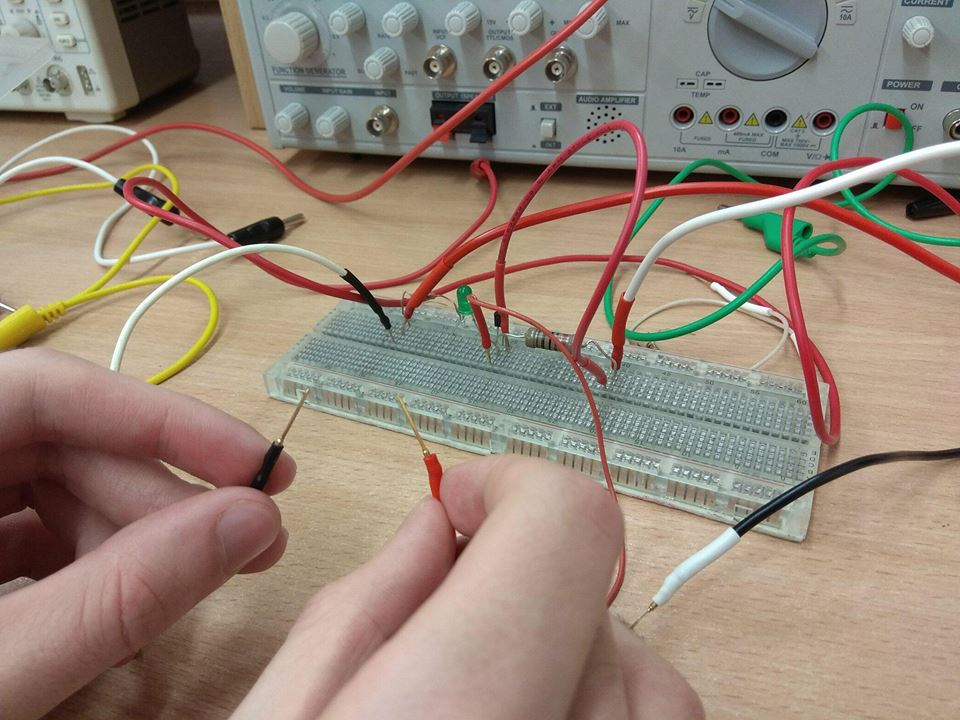
\includegraphics[scale=0.4]{dioda1rozwarte.jpg}
	\captionof{figure}{Układ pomiarowy przy rozwartych zaciskach $A-A$}
\end{figure}

\begin{figure}[H]
	\centering
	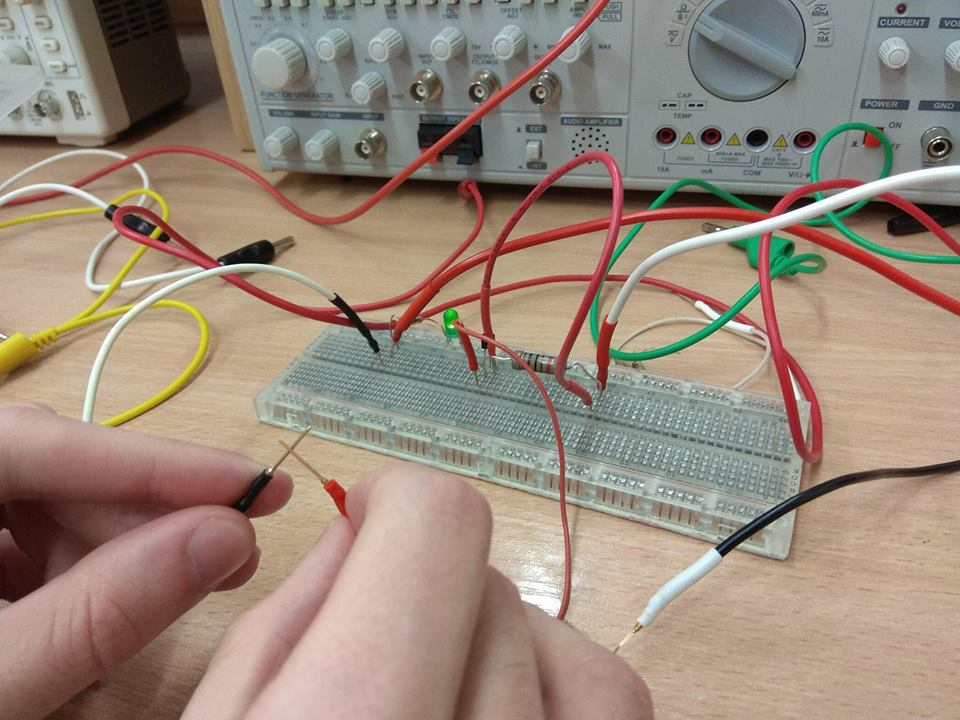
\includegraphics[scale=0.4]{dioda1zwarte.jpg}
	\captionof{figure}{Układ pomiarowy przy zwartych zaciskach $A-A$}
\end{figure}

Następnie rozbudowano układ według poniższego schematu i zaobserwowano działanie układu po zwarciu wyprowadzeń $A-A$.


%%  rys 1.15.
\begin{figure}[H]
	\begin{equation*}
	\begin{circuitikz}[american]
	\draw
	(0,0) to (6,0)
	to [V,v=$10V$] (6,3)
	(6,3) to  [european resistor, a = $R_{13}$, l= $1k\Omega$](4,3)
	(2,3) to [leD-,invert , a =LED2] (4,3)
	(2,2) node[nmos] (mos) {}
	(mos.drain) node[anchor = east] {D}
	(mos.source) node[anchor = east] {S}
	(mos.gate) node[anchor = south] {G}
	(2,3) to (mos.drain)
	(2,0) to (mos.source)
	(mos.gate) to (0,2)
	(0,2) to [european resistor, a =$R_{14}$, l=$47k\Omega$] (0,0)
	(0,0) to (-3,0)
	to [C,l=$C1$,a=$100 \mu F$] (-3,2)
	to (0,2)
	(-3,2) to [short, -*] (-4,2)
	(6,3) to (6,4.5)
	to (-4,4.5)
	to [short,-*](-4,3)
	(-4,2.5) node[anchor = mid] {A-A};
	\end{circuitikz}
	\end{equation*}
	\captionof{figure}{Model układu z opóźnionym wyłączaniem}
\end{figure}



\begin{figure}[H]
	\centering
	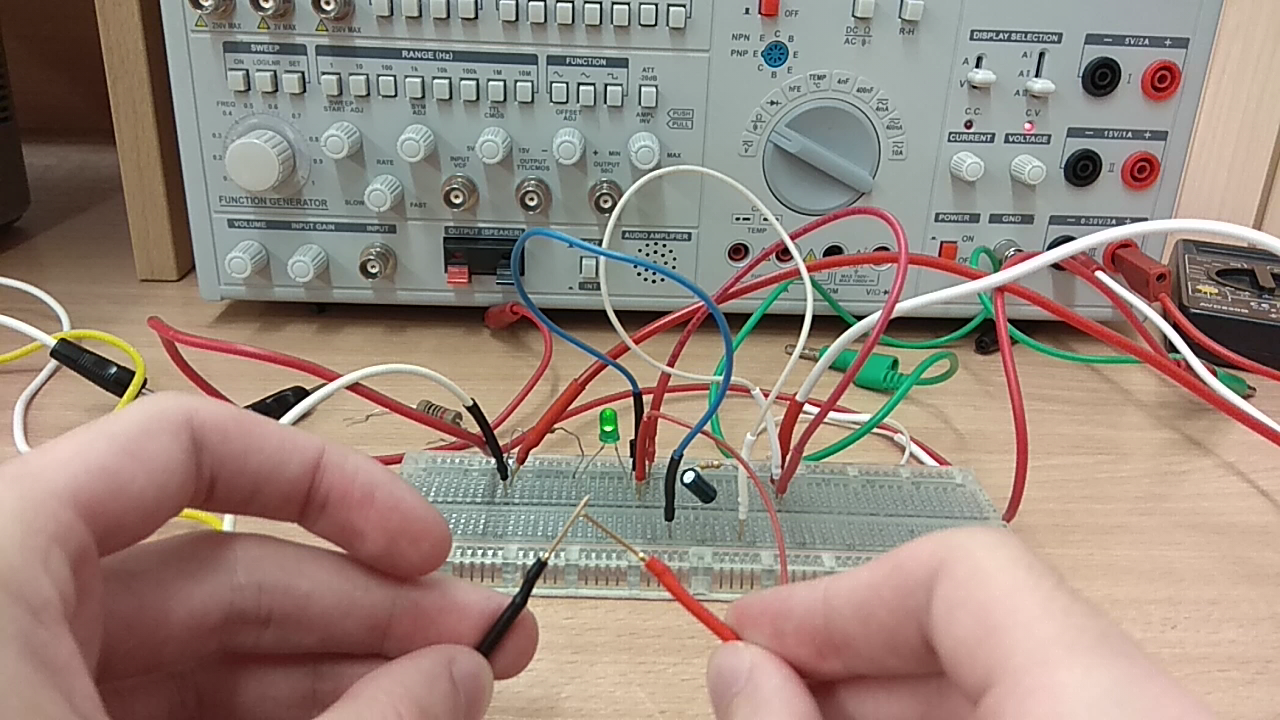
\includegraphics[scale=0.3]{1.png}
	\captionof{figure}{Układ pomiarowy przy zwartych zaciskach $A-A$}
\end{figure}

\begin{figure}[H]
	\centering
	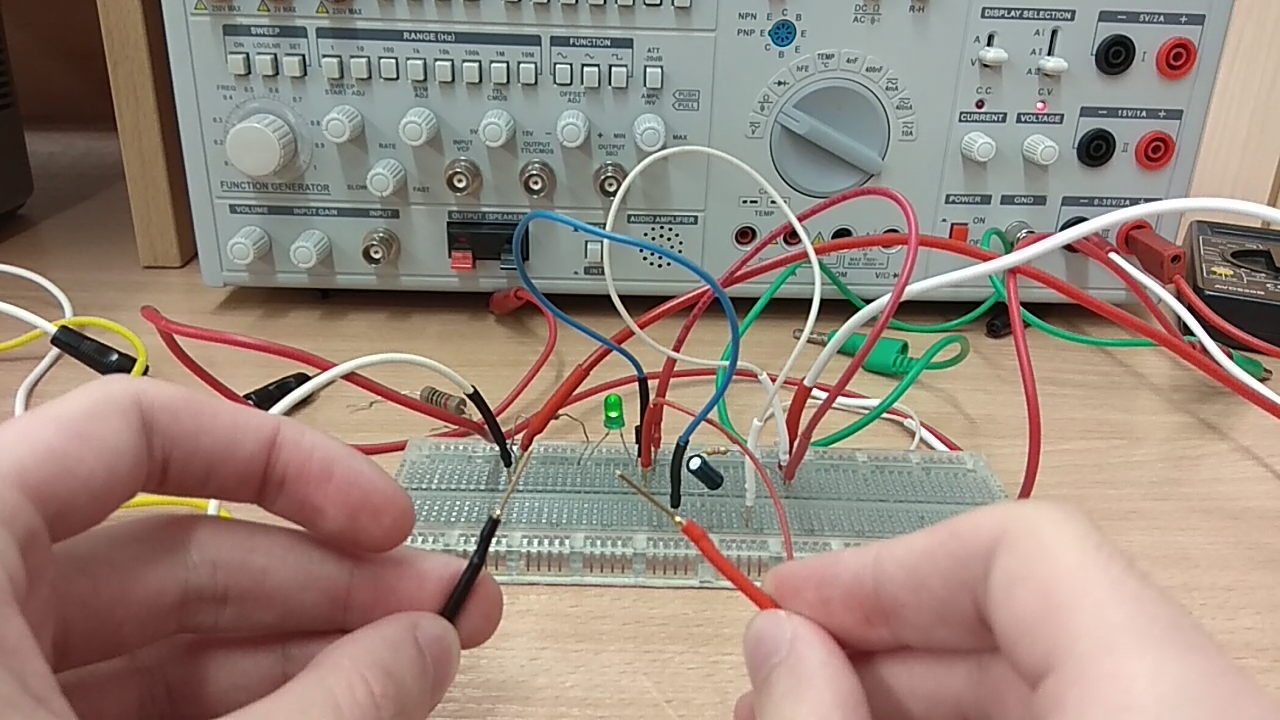
\includegraphics[scale=0.3]{2.png}
	\captionof{figure}{Układ pomiarowy, po upływie 1 sekundy od rozwarcia zacisków $A-A$}
\end{figure}

\begin{figure}[H]
	\centering
	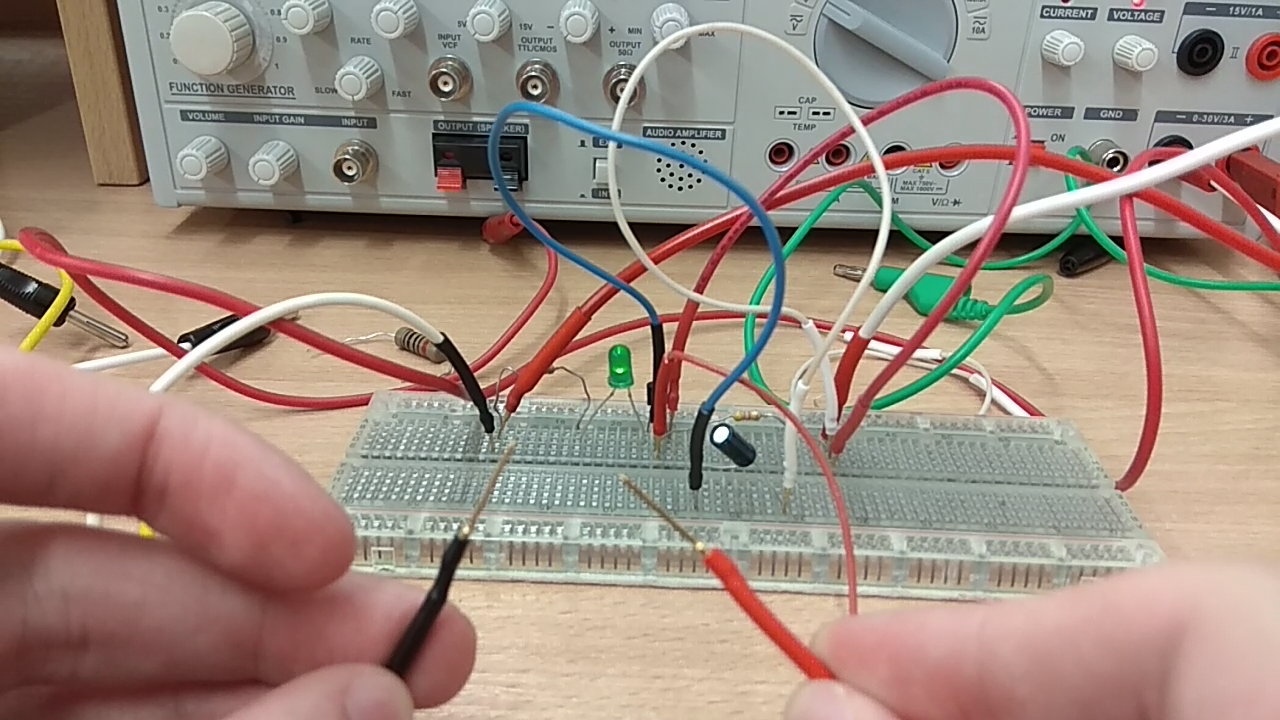
\includegraphics[scale=0.3]{3.png}
	\captionof{figure}{Układ pomiarowy, po upływie 4 sekund od rozwarcia zacisków $A-A$}
\end{figure}

\begin{figure}[H]
	\centering
	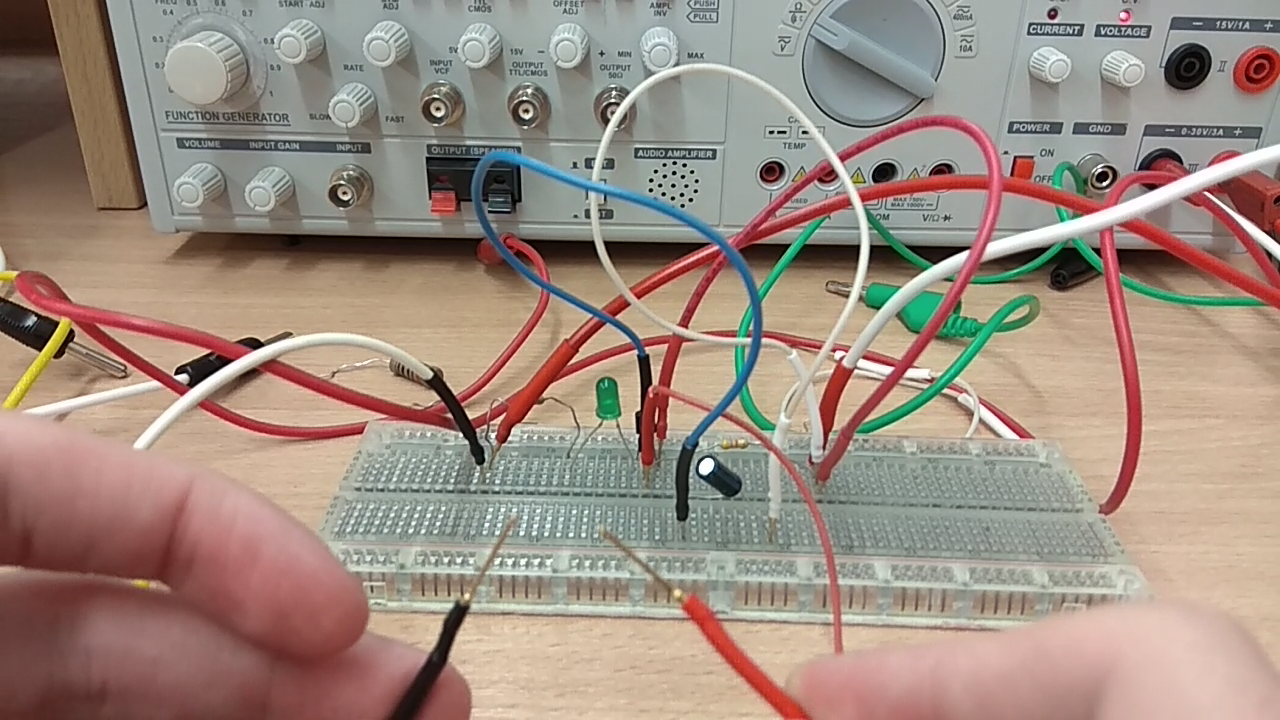
\includegraphics[scale=0.3]{4.png}
	\captionof{figure}{Układ pomiarowy, po upływie 5 sekund od rozwarcia zacisków $A-A$}
\end{figure}

\subsection{Wnioski}

Dioda z drugiego układu po zwarciu zacisków zaczęła świecić, a po ich rozwarciu przez około $ 3.5 $ sekundy świeciła z taką samą intensywnością, następnie powoli przygasała, aby po upływie około $ 4.5 $ sekundy zgasła całkowicie. Aplikacją praktyczną takiego urządzenia może być na przykład użycie go w czytniku kart dostępu, po przyłożeniu i odczytaniu karty zapali się dioda LED o odpowiednim kolorze, a po upływie pewnego czasu zgaśnie. 

\section{Czas załączania tranzystora}

\subsection{Cel zadania}
Badanie wpływu prostokątnego przebiegu sterującego na działanie diody.
\subsection{Przebieg zadania}

Zbudowano obwód przedstawiony poniżej.

%%  rys 1.17.
\begin{figure}[H]
	\begin{equation*}
	\begin{circuitikz}[american]
	\draw
	(0,0) to (6,0)
	to [V,v=$10V$] (6,3)
	(6,3) to  [european resistor, a = $R_{15}$, l= $1k\Omega$](4,3)
	(2,3) to [leD-, invert, a = LED3] (4,3)
	(2,2) node[nmos] (mos) {}
	(2,3) to (mos.drain)
	(2,0) to (mos.source)
	(mos.gate) to (0,2)
	(0,2) to [european resistor, a =$R_{16}$, l=$1M\Omega$] (0,0)
	(0,0) to (-2,0)
	to [sV,l=BNC] (-2,2)
	to (-2,2)
	(-2,0) node[ground]{}
	(-2,2) to (0,2);
	\draw [red]
	(-2,2) to (-2,6)
	(2,3) to (2,4.5)
	to (6,4.5)
	(4,4.75)node[anchor = mid] {Czerwony kabel z kanału Y oscyloskopu}
	(-2.25,5)node[anchor = mid,rotate = 90] {Czerwony kabel z kanału X oscyloskopu};
	\draw
	(-0.25,5.5)node[anchor = mid,rotate = 90] {Czarny kabel z kanału X oscyloskopu}
	(4,6)node[anchor = mid] {Czarny kabel z kanału Y oscyloskopu}
	(0,6) to (0,3)
	(0,3) node[ground] {}
	(6,5.5) to (2,5.5)
	(2,5.5) node[ground,rotate =270] {};	
	\end{circuitikz}
	\end{equation*}
	\captionof{figure}{Obwód do pomiaru czasu przełączania}
\end{figure}

Wykonano polecenia z pliku pdf przedstawionego przez prowadzącego i zaobserwowano zmiany w wypełnieniu prostokątnego przebiegu sterującego i jego wpływ na intensywność świecenia diody LED.

\begin{figure}[H]
	\centering
	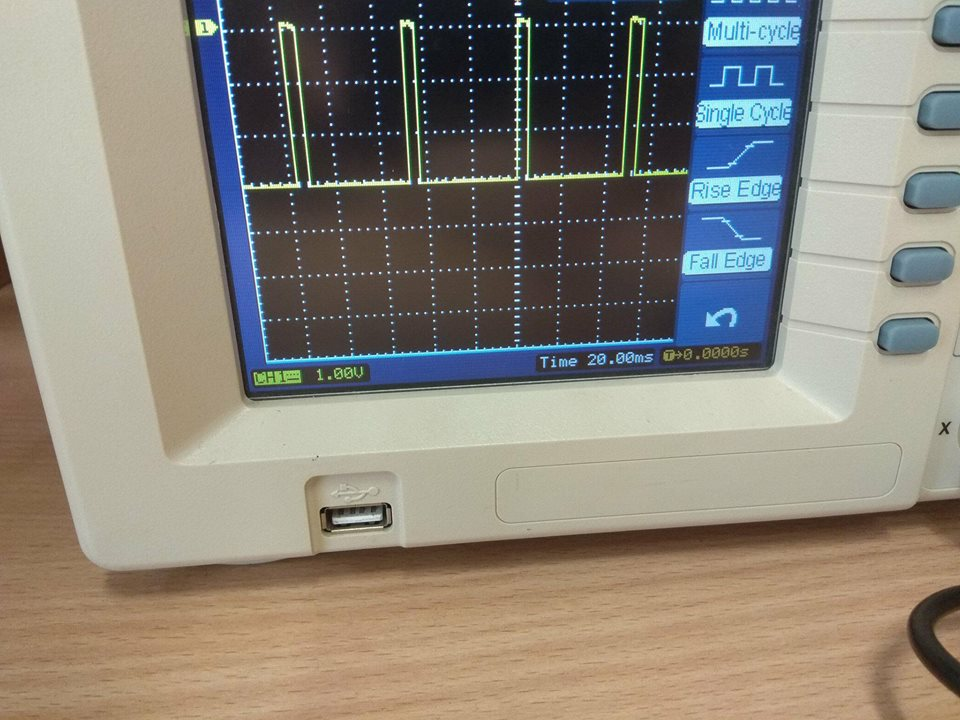
\includegraphics[scale=0.3]{male.jpg}
	\captionof{figure}{Male wypełnienie}
\end{figure}

\begin{figure}[H]
	\centering
	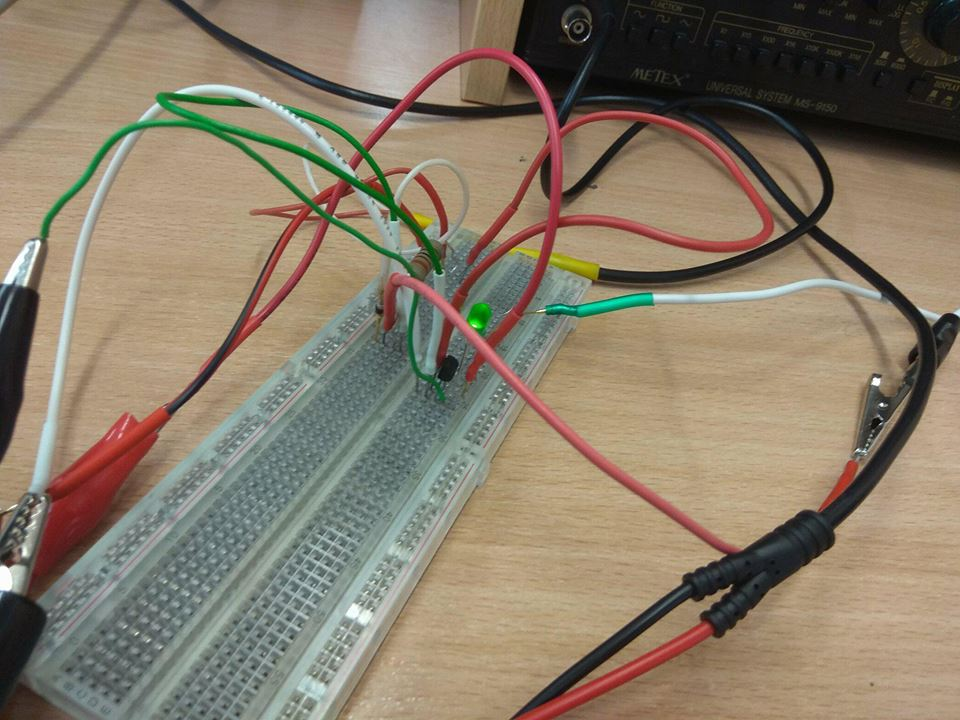
\includegraphics[scale=0.3]{diodadlamalego.jpg}
	\captionof{figure}{Duże wypełnienie}
\end{figure}

\begin{figure}[H]
	\centering
	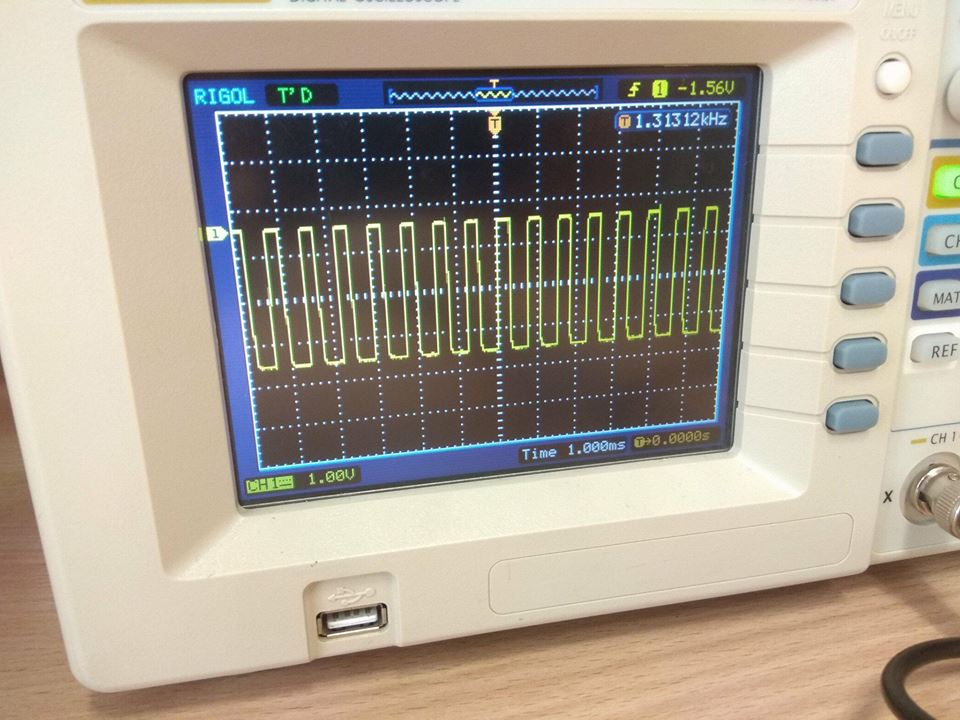
\includegraphics[scale=0.3]{duze.jpg}
	\captionof{figure}{Duże wypełnienie}
\end{figure}

\begin{figure}[H]
	\centering
	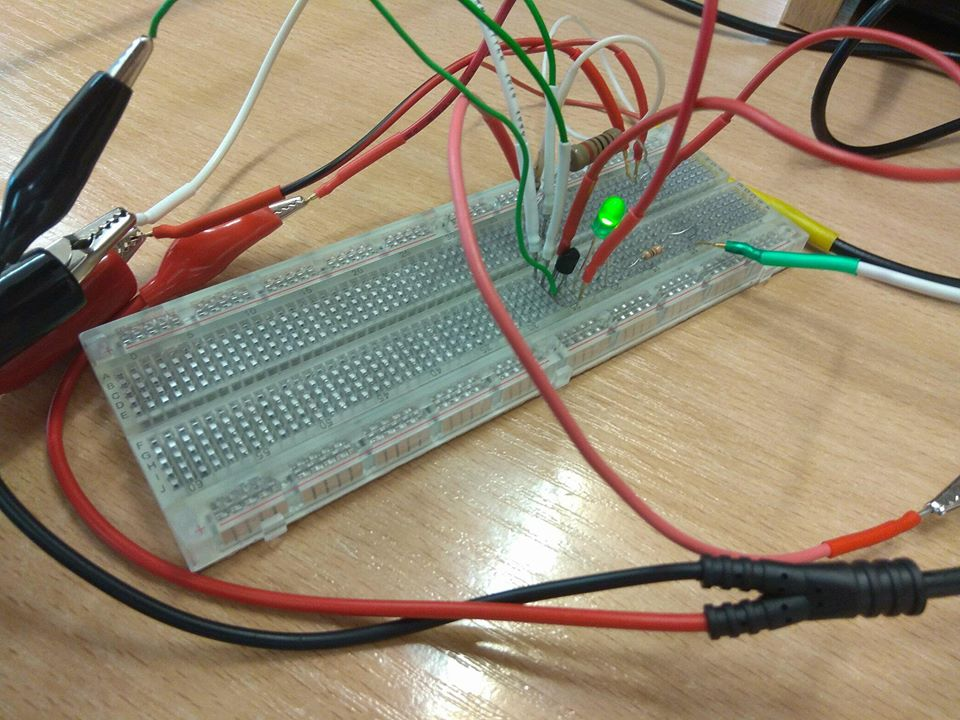
\includegraphics[scale=0.3]{diodadladuzego.jpg}
	\captionof{figure}{Duże wypełnienie}
\end{figure}

\subsection{Wnioski}

Wraz ze wzrostem wypełnienia prostokątnego przebiegu sterującego intensywność świecenia diody rośnie, a z jego spadkiem maleje.

\subsection{Cel zadania}
Oszacowanie maksymalnej stabilnej częstotliwości pracy układu tranzystora i diody LED.

\subsection{Przebieg zadania}

Po podniesieniu częstotliwości pobudzenia ponad 1MHz, oscyloskop nie wskazał przewidywanych wyników, a prowadzący uznał, że to wina generatora. Po przeniesieniu się na inne stanowisko i użyciu innego generatora oscyloskop dalej nie wskazywał przewidywanych wartości, prowadzący potwierdził poprawne złożenie układu i użycia oscyloskopu.


Jeśli udałoby się uzyskać prawidłowe wyniki, określono dla jakiej częstotliwości zostały utworzone i zapisano szacowany czas przełączenia $t_{d}$, a następnie przy pomocy wzoru $f_{max} = \dfrac{1}{t_{d}}$ obliczono maksymalną stabilną częstotliwość pracy układu tranzystora i diody LED.

	\begin{thebibliography}{99}
		\bibitem{pa}Encyclopaedia Britannica http://www.britannica.com/, 
		
		\bibitem{pa1}BS170/MMBF170 \emph{0 N-Channel Enhancement Mode Field Effect Transistor, National Semiconductor}. 1992r.
		
		\bibitem{pa2}TP0610L/T, VP0610L/T \emph{BS250 P-Channel 60-V (D-S) MOSFET, Vishay Siliconix.} 2001r.

		\bibitem{pa4} ADI \emph{, Sztuka elektroniki, tomy 1. i 2, } WKiŁ, Warszawa 2003r.
		
		\bibitem{pa5}] ] Resnick R., Halliday D., Walker J.,  \emph{Podstawy fizyki, tom 3.,} PWN, Warszawa 2003r.
		
		\bibitem{pa6}] Watson J. \emph{ Elektronika,} WKiŁ, Warszawa 1999r.
		
		\bibitem{pa7}Nosal Z., Baranowski J. \emph{Układy elektroniczne,} Warszawa 2003r.
	\end{thebibliography}
		
	\newpage
	\tableofcontents
		
\end{document}


